% 2D Vector Subtraction
%
% File:         2d-vector-subtraction.tex
% Author:       Bob Walton (walton@acm.org)
% Date:      	Sun Dec 23 06:54:48 EST 2012
  
\documentclass{minimal}
\usepackage[paperheight=2.4in,paperwidth=2in,
            height=2.4in,hoffset=0.05in,
	    voffset=0.05in,left=0in,width=2in]{geometry}
\usepackage{color}
\usepackage[usenames]{xcolor}
\usepackage{scalefnt}
\usepackage{tikz}
\newcommand{\SMALL}{\scalefont{0.8}}
\usetikzlibrary{arrows}
\begin{document}
\raggedright
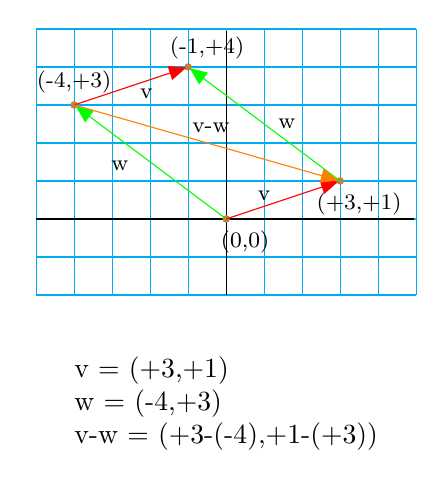
\begin{tikzpicture}[x=0.190in,y=0.190in]
\begin{scope}[yshift=1in,>=triangle 45,shorten >=0.01in]
    \draw[cyan] (-5,-2) grid[step=1] (5,5);
    \draw[black] (-5,0) -- (+5,0);
    \draw[black] (0,-2) -- (0,+5);

    \fill[brown] (0,0) circle(0.1) + (+0.5,-0.6) node[black]{\SMALL (0,0)};

    \draw[red,->] (0,0) -- (+3,+1);
    \draw[black] (1.0,0.6) node{\SMALL v};
    \fill[brown] (+3,+1) circle(0.1) + (+0.5,-0.6) node[black]{\SMALL (+3,+1)};
    \draw[green,->] (+3,+1) -- (-1,+4);
    \draw[black] (+1.6,2.5) node{\SMALL w};
    \fill[brown] (-1,+4) circle(0.1) + (+0.5,+0.5) node[black]{\SMALL (-1,+4)};

    \draw[green,->] (0,0) -- (-4,+3);
    \draw[black] (-2.8,1.4) node{\SMALL w};
    \fill[brown] (-4,+3) circle(0.1) + (+0.0,+0.6) node[black]{\SMALL (-4,+3)};
    \draw[red,->] (-4,+3) -- (-1,+4);
    \draw[black] (-2.1,3.3) node{\SMALL v};

    \draw[orange,->] (-4,+3) -- (+3,+1);
    \draw[black] (-0.4,2.4) node{\SMALL v-w};
\end{scope}

\begin{scope}
\draw (0,0.4) node {
    \begin{tabular}[t]{l}
    v = (+3,+1) \\
    w = (-4,+3) \\
    v-w = (+3-(-4),+1-(+3)) \\
    \end{tabular}
    };
\end{scope}
\end{tikzpicture}
\end{document}
